% !TEX root = robobrain.tex
\section{Applications}
\label{sec:applications}
In this section we first show how \robobrain{} can be used \textit{as-a-service} by the robots for several robotics problems. Specifically, we explain the usage of \robobrain{} in anticipating human activities, grounding of natural language sentences, and path planning. We then show how \robobrain{} can help robotics projects by sharing knowledge within the projects and throughout the Internet.

\subsection{\robobrain{} \textit{as-a-service}}
Our goal with providing \robobrain{} \textit{as-a-service} is to allow robots to use the representations learned by different partner projects. 
% For this purpose the 
% RKE stores the representations learned by different projects, allows queries through RQL. 
This 
% feature of the RKE 
allows \robobrain{} to effortlessly address many robotics applications. In the following we demonstrate \robobrain{} as-a-service feature for three robotics applications that deal with different data modalities of perception, natural language and trajectories.

% !TEX root = ../../ozan_sener_thesis.tex
\begin{figure}
\centering
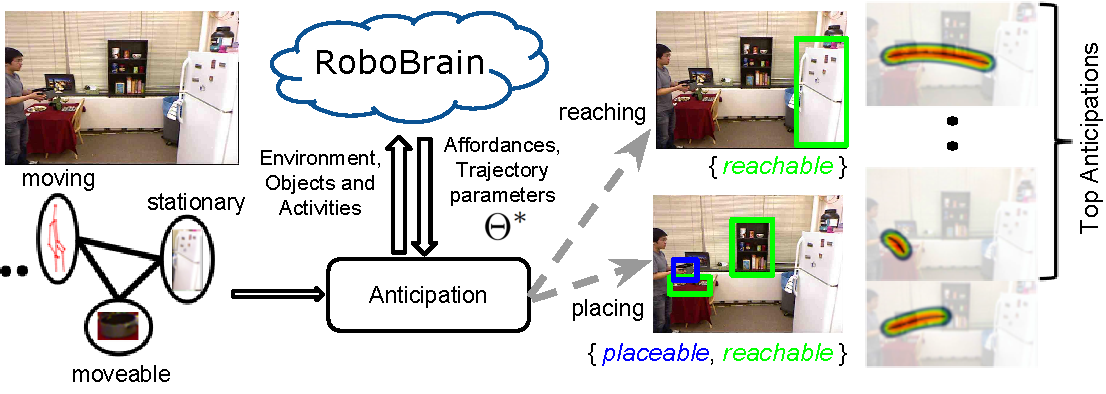
\includegraphics[width=\linewidth]{./Image/anticipation_robobrain_pic.pdf}
\caption{\textbf{\robobrain{} for anticipating human activities.} Robot using anticipation algorithm of \citet{KoppulaRSS2013} queries \robobrain{}, for the activity, affordance and trajectory parameters in order to generate and rank the possible future activities in a given environment.}
\label{Fig:anticipation}
\end{figure}

\subsubsection{Anticipating human actions}
\label{sec:anticipation}
The assistive robots working with humans should be able to understand human activities and also anticipate the future actions that the human can perform. In order to anticipate, the robot should reason over the action possibilities in the environment, i.e., \textit{object affordances}, and how the actions can be performed, i.e., \textit{trajectories}. Several works in robotics have addressed the problem of anticipation~\citep{KitaniECCV2012,KoppulaRSS2013,Kuderer-RSS-12}.

We now show how robots can query \robobrain{} and use the previous work by
Koppula et al.~\citep{KoppulaRSS2013} for anticipating human actions.  
In order to anticipate the future human actions, the authors~\citep{KoppulaRSS2013} learn parameters using their anticipatory algorithm, and using the learned parameters they anticipate the most likely \textit{future} object affordances and human trajectories. \robobrain{} serves anticipation \textit{as-a-service} by storing those learned parameters, object affordances and trajectories  as concepts in its graph. Figure~\ref{Fig:anticipation} illustrates a robot retrieving relevant information for anticipation. The robot first uses the following queries to retrieve the possible trajectories of an object:

%\noindent \resizebox{\linewidth}{!}{
%\begin{minipage}{\linewidth}
{\small
\begin{align}
&{\tt {affordances} \,\, n := fetch \,\,(\{name:n\})\rightarrow   [`HasAffordance'] \rightarrow } \cr
& {\tt \hspace*{2cm} (v\{src:`Affordance'\})   \nonumber } \\
&{\tt {trajectories} \,\, a := fetch \,\,(\{handle:a\})\rightarrow [`HasParameters']\rightarrow } \cr
& {\tt \hspace*{2cm}  (v\{src:`Affordance', type:`Trajectory'\})  \nonumber } \\
& {\tt { trajectory\_parameters} \,\, o := \,\, } \cr
&{\tt \hspace*{2cm} map (\lambda a \rightarrow {trajectories}\,\, a)  \,\, {affordances}\,\, o } \nonumber
\end{align}
%  \end{minipage}
}


In the queries above, the robot first queries for the affordances of the object and then for each affordance it queries \robobrain{} for the trajectory parameters. Having retrieved all possible trajectories, the robot uses the learned parameters~\citep{KoppulaRSS2013} to anticipate the future human actions. Since the learned parameters are also stored in the \robobrain{} graph, the robot retrieves them using the following RQL queries:
{\small
\begin{align*}
&{\tt {parents} \,\, n := fetch \,\, (v)\rightarrow [`HasParameters']\rightarrow  (\{handle:n\}) }\nonumber \\
& {\tt {parameters} \,\, n :=  fetch \,\, (\{name:n\})\rightarrow [`HasParameters']\rightarrow }\cr
& {\tt \hspace*{2cm}  (v\{src:`Activity'\})   \nonumber } \\
& {\tt find\_parameters\, a := }\\
& \hspace*{2cm}{\tt filter (\lambda u \rightarrow\! {Len\; parents}\, u = 1)     {parameters}\, a \nonumber } \\
& {\tt {joint\_parameters} \,\, a_1 \,\, a_2\,\, := filter (\lambda u \rightarrow {Len\; parents}\,\, u = 2\,\, } \cr
& {\tt \hspace*{2cm}  and\,\, u \,\, in \,\, {parameters}\,\, a_2)    \,\,{parameters}\,\, a_1 \nonumber}
\end{align*}
}
The queries above retrieves both independent and joint parameters for anticipating the object affordances and human activities. Detailed explanation of the query is given in Example \ref{ex:joint} of Section \ref{sec:raquel}



% !TEX root = robobrain.tex

\subsubsection{Grounding natural language} The problem of grounding a natural language instruction in an environment requires the robot to formulate an action sequence  that accomplish the semantics of the  instruction~\citep{tellex2011understanding,misra2014tell,guadarrama2013grounding, MatuszekISER2012}. In order to do this, the robot needs a variety of information. Starting with finding action verbs and objects in the instruction, the robot has  to discover those objects and their affordances in the environment.

% \robobrain{} provides natural language grounding \textit{as-a-service}.

We now show the previous work by Misra et al.~\cite{misra2014tell} using \robobrain{} \textit{as-a-service} in their algorithm. In order to ground a natural language instruction the robot has to check for the satisfiability of the actions it generates in the given environment. For example, an action which pours water on a book should be deemed unsatisfiable. In the previous work~\cite{misra2014tell}, the authors manually define many pre-conditions to check the satisfiability of actions. For example, they define manually that a \textit{syrup bottle} is \textit{squeezable}. Such satisfiability  depends on the object's affordances in the given environment, which can be retrieved from \robobrain{}.

Figure~\ref{Fig:languagegrounding} illustrates a robot querying \robobrain{} to check the satisfiability of actions that it can perform in the given environment. Below is the RQL query for retrieving the satisfiability of  \textit{squeezable} action:
%\noindent \resizebox{\linewidth}{!}{
%\begin{minipage}{\linewidth}
{\small
\begin{align*}
&{\tt {squeezable \,\ syrup}\,\,  := \,\,Len \,\,fetch \,\,(u\{name:`syrup'\})\rightarrow }\\
&{\tt \hspace*{0.1cm} [`HasAffordance']\rightarrow (v\{name:`squeezable'\})\,\,> 0}
\end{align*}
%  \end{minipage}
}

\begin{figure}[t]
\centering
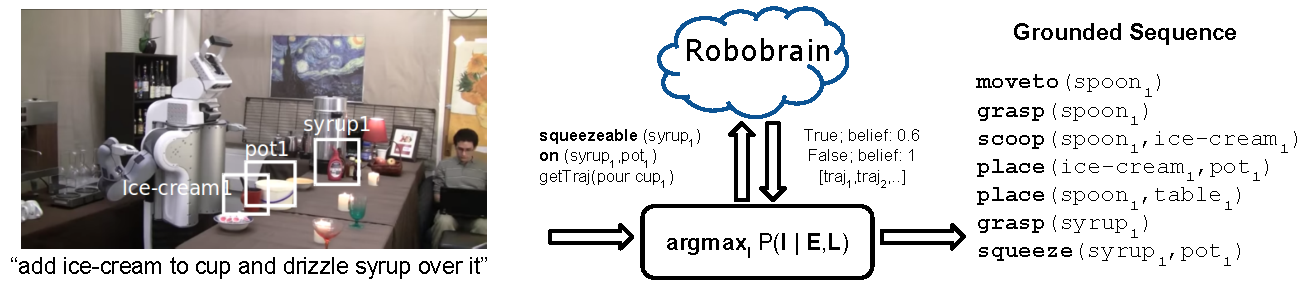
\includegraphics[width=1\linewidth]{./Image/tellmedave_robobrain_pic.pdf}
\caption{\textbf{Grounding natural language sentence.} The robot grounds natural language by using the algorithm by Misra et al.~\cite{misra2014tell} and querying \robobrain{} to check for the satisfiability of actions.}
%\cite{misra2014tell} requires several  pieces of knowledge. Robot should know the appearances and affordances of objects, as well as the possible actions related to each object and it should know the trajectories and manipulation features of those actions. These are all  translated as queries to the RKE graph.}
\label{Fig:languagegrounding}
\end{figure}
% !TEX root = robobrain.tex
\subsubsection{Path planning using \robobrain{}}
\label{sec:applicationplanit}

One key problem robots face in performing tasks in human environments is identifying trajectories desirable to the users. An appropriate trajectory not only needs to be valid from a geometric standpoint (i.e., feasible and obstacle-free), but it also needs to satisfy the user preferences~\citep{jainsaxena2013_trajectorypreferences,Jain14}. For example,  a robot should move sharp objects such as knife strictly away from nearby humans~\cite{jain_contextdrivenpathplanning_2013}. Such preferences are commonly represented as cost functions which jointly model the environment, the task, and trajectories.
%This joint modeling is expensive in terms of resource requirement (e.g., robots) and data collection, and
Typically research groups have independently learned different cost functions~\citep{jainsaxena2013_trajectorypreferences,Kuderer-RSS-12,KitaniECCV2012}, which are not shared across the research groups. Here we show \robobrain{} \textit{as-a-service}  for a robot to store and retrieve the planning parameters.
%We now show how the previous work by Jain et al.~\citep{Jain14} use the RKE for retrieving the trajectory parameters for path planning. We demonstrate this on the example of moving an egg carton from the previous work~\citep{Jain14}.

In Figure~\ref{fig:planning} we illustrate the robot planning for an egg carton by querying \robobrain{}.
Since eggs are \textit{fragile}, users  prefer to move them slowly and close to the surface of the table.  In order to complete the task, the robot queries \robobrain{} and retrieves the attributes of the egg carton and also the trajectory parameters learned in the previous work by Jain et al.~\citep{Jain14}. Using the retrieved attributes and the parameters, the robot samples trajectories and executes the top-ranked trajectory.
%need labels of all objects in the environment. In this example we use the
%object labels provided by the authors~\cite{Jain14}. After the object labels are obtained, the previous
%work~\citep{Jain14} use the RKE to retrieve attributes of the egg carton and also the trajectory
%parameters.
Below we show the RQL queries.
%\noindent \resizebox{\linewidth}{!}{
%\begin{minipage}{\linewidth}
{\small
\begin{align*}
&{\tt {attributes} \,\, n := fetch \,\,(\{name:n\})\rightarrow
[`HasAttribute'] \rightarrow (v)   \nonumber} \\
&{\tt {trajectories} \,\, a := }\\
&{\tt\hspace*{2cm} fetch \,(\{handle :a\})\rightarrow  [`HasTrajectory'] \rightarrow (v)  \nonumber } \\
&{\tt {trajectory\_parameters} := }\\
&{\tt \hspace*{2cm} map (\lambda a \rightarrow
{trajectories}\,\, a)  \,\, {attributes}\,\, `egg' } \nonumber
\end{align*}
%  \end{minipage}
}

\begin{figure}[t]
\centering
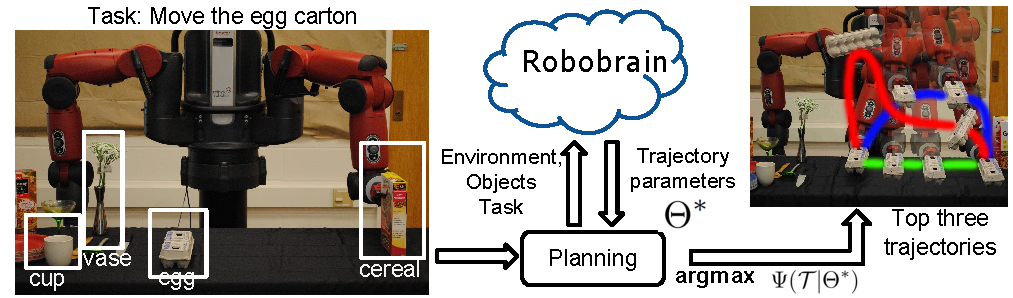
\includegraphics[width=\linewidth]{Image/planit_robobrain_pic_2}
\caption{\textbf{\robobrain{} for planning trajectory.} The robot queries \robobrain{} for the trajectory parameters (learned by Jain et al.~\citep{jainsaxena2013_trajectorypreferences})  to plan paths for the fragile objects like an egg carton. }
\label{fig:planning}
\end{figure}

% !TEX root = ../../ozan_sener_thesis.tex


\subsection{\robobrain{} for sharing knowledge}
\robobrain{} allows sharing the knowledge learned by different research groups as well as knowledge obtained from various internet sources. In this section we show with experiments how sharing knowledge improves existing robotic applications:

\iffalse
\subsubsection{Sharing knowledge from the Internet}
In this experiment we show that sharing knowledge from several Internet sources using \robobrain{} improves robotic applications such as path planning.  Knowledge from the Internet sources has been shown to help robots in planing better paths~\citep{beetzIcra2010}, understand natural language~\citep{coyneCosli,tellex2011understanding}, and also recently in object retrieval~\citep{guadarramaRss2014}. However, for certain robotic tasks a single Internet source does not cover many of the real world situations that the robot may encounter. In such situations it is desired to share the information from other sources to get an overall richer representation.
The \robobrain{} graph is designed to acquire and connect information from multiple Internet sources and make it accessible to robots.

In this experiment we build upon work by Jain et al.~\citep{jainsaxena2013_trajectorypreferences} for planning trajectories that follow user preferences. The work relied on object attributes in order to plan desirable trajectories. These attributes convey properties such as whether an object is sharp, heavy, electronic etc. The attributes were manually defined by the authors~\citep{jainsaxena2013_trajectorypreferences}. In practice this is very challenging and time-consuming because there are many objects and many attributes for each object.
%Jain et al.~\citep{jainsaxena2013_trajectorypreferences}  manually define attributes used by TPP.
Instead of manually defining the attributes, we can retrieve many of them from the Internet knowledge
sources such as OpenCyc, Wikipedia, etc. However, a single knowledge source might not have
attributes for all objects.
The \robobrain{} graph connects many attributes obtained from multiple Internet sources to their respective objects.
%We crawl multiple internet sources to retrieve many attributes and connect them to their respective objects in the \robobrain{} graph.


\begin{figure}
\centering
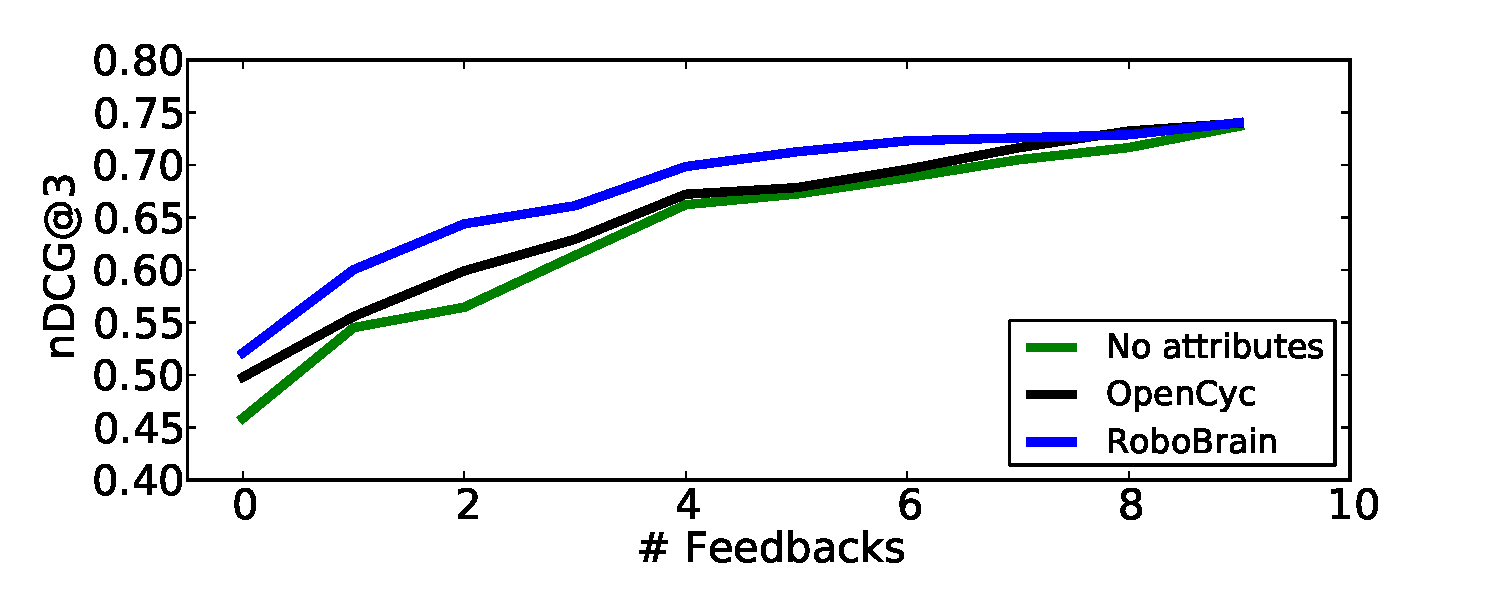
\includegraphics[width=\linewidth]{Image/internet_attributes}
\caption{\textbf{Sharing from Internet sources.} The plot shows performance of  the algorithm by Jain et al.~\citep{jainsaxena2013_trajectorypreferences} for three settings of attributes. This is an online algorithm that learns a good trajectory from the user feedback. The performance is measured using the nDCG metric~\cite{manning2008introduction}, which represents the quality of the ranked list of trajectories. \robobrain{} combines information from multiple sources and hence its richer in attributes as compared to retrieving attributes from OpenCyc alone.}
\label{fig:ndcg}
\end{figure}

Figure~\ref{fig:ndcg} illustrates the planning results when the robot does not use any attributes, when it uses attributes from a single source (OpenCyc), and when it use attributes from \robobrain{}. The planning performance is best when using \robobrain{} since it covers more attributes than the OpenCyc alone. Most importantly all these attributes are retrieved from the \robobrain{} graph with a single RQL query as explained in Section \ref{sec:applicationplanit}.
\fi

%\subsubsection{Sharing learned representations}

New algorithms are commonly proposed for a problem to address the shortcomings of previous methods. These algorithms have their own learned representations. For example,  different representations  have been learned for grounding natural language~\citep{tellex2011understanding,misra2014tell,guadarrama2013grounding, MatuszekISER2012}. However, it is usually hard for practitioners to choose a single representation since there are always inputs where one representation fails but some others work. In this experiment we show that a robot can query \robobrain{} for the best representation while being agnostic to the algorithmic details of the learned representations.

Simulating the above setting, we present an experiment for sharing multiple learned representations on a natural language grounding problem. Here the goal is  to output a sequence of instructions for the robot to follow, given an input natural language command and an environment.
Following the work by Misra et al.~\citep{misra2014tell}, we train a baseline algorithm for the task of \textit{making ramen} (Algorithm A), and train their full algorithm for the task of \textit{making affogato} (Algorithm B). These algorithms assign a  confidence score (i.e., probability) to the output sequence of instructions.  We store these learned representations as concepts in the \robobrain{} graph, along with a prior belief over the correctness of the algorithms. The robot queries \robobrain{} for a representation as follows:
%\resizebox{\linewidth}{!}{
%\begin{minipage}{\linewidth}
{\small
\begin{align*}
& {\tt algParam  :=  fetch (u\{type:'GroundingAlgorithm'\})}\rightarrow \\
& {\tt \hspace*{2cm} [`HasParameters'] \rightarrow (v)}   \\
& {\tt prior \,\, n :=  fetch (\{name:n\})\rightarrow [`HasPriorProb'] \rightarrow (v)}\\
& {\tt groundings \,\, L,E :=   argMaxBy(\lambda(u,v)\rightarrow v)} \\
& {\tt \hspace*{2cm} map(\lambda(u,v) \rightarrow u(L,E,v)*prior\, u) \, \, \, algParam}
\end{align*}
%\end{minipage}
}

\medskip
In the ${\tt algParam}$ function, we retrieve all natural language grounding algorithms from the \robobrain{} graph with their parameters. This returns a list in which each element is a tuple of algorithm $u$ and its parameters $v$. The ${\tt prior}$ function retrieves the prior belief over the correctness of an algorithm. In order to ground a given natural language command ${\tt L}$ in environment ${\tt E}$, the ${\tt grounding}$ function evaluates the likelihood score for each algorithm  using their parameters as ${\tt u(L,E,v)}$. It further incorporates the prior belief over the algorithms, and returns the representation with the highest likelihood score. These set of queries corresponds to the following likelihood maximization equation:
\begin{equation*}
\mathcal{I}^*  = \argmax_{\mathcal{I},m'\in \{A,B\}} P(\mathcal{I}|E, L,  w_{m'}^* ,m')P(m')
\end{equation*}
As shown in the Table~\ref{tbl:grounding-results}, choosing a representation by querying the \robobrain{} achieves better performance than the individual algorithms.

\begin{table}
\caption{\robobrain{} allows sharing learned representations. It allows the robot to query \robobrain{} for a representation given an input natural language command. In this table the Algorithm $A$ is a greedy algorithm based on Misra et al.~\cite{misra2014tell}, and Algorithm $B$ is their full model. The $IED$ metric measures the string-edit distance and the $EED$ metric measures the semantic distance between the ground-truth and the inferred output instruction sequences. The metrics are normalized to 100 such that higher numbers are better.}
\label{tbl:grounding-results}
\centering
\begin{tabular}{l|cc}
\hline
\textbf{Algorithm} & \textbf{IED} & \textbf{EED}\\
\hline
Algorithm A & 31.7 & 16.3\\
Algorithm B & 23.7 & \textbf{27.0}\\
\robobrain{} (A+B) & \textbf{34.2} & 24.2\\
\hline
\end{tabular}
\end{table}

